\documentclass[UTF8]{article}
\usepackage{graphicx}
\usepackage{subfigure}
\usepackage{amsmath}
\usepackage{makecell}
\usepackage[utf8]{inputenc}
\usepackage[space]{ctex} %中文包
\usepackage{listings} %放代码
\usepackage{xcolor} %代码着色宏包
\usepackage{CJK} %显示中文宏包
\usepackage{float}
\usepackage{diagbox}
\usepackage{bm}
\usepackage{ulem} 
\usepackage{amssymb}
\usepackage{soul}
\usepackage{color}
\usepackage{geometry}
\usepackage{fancybox} %花里胡哨的盒子
\usepackage{xhfill} %填充包, 可画分割线 https://www.latexstudio.net/archives/8245
\usepackage{multicol} %多栏包
\usepackage{enumerate} %可以方便地自定义枚举标题
\usepackage{multirow} %表格中多行单元格合并
\usepackage{wasysym} %可以使用wasysym里的一堆奇奇怪怪的符号
\usepackage{hyperref} % url
%%%%%%%%%%%%%%%伪代码%%%%%%%%%%%%%%%
\usepackage{amsmath}
\usepackage{algorithm}
\usepackage{algorithmicx}
\usepackage[noend]{algpseudocode}
%%%%%%%%%%%%%%%画图包%%%%%%%%%%%%%%%
\usepackage{tikz}
\usepackage{pgfplots} % http://pgfplots.sourceforge.net/gallery.html
\usetikzlibrary{pgfplots.patchplots} % 拟合支持
\usetikzlibrary{arrows,shapes,automata,petri,positioning,calc} % 状态图支持
\usetikzlibrary{arrows.meta} % 箭头
\usetikzlibrary{shadows} % 阴影支持
\usepackage{forest} % 画树

\geometry{left = 2cm, right = 2cm, top=2cm, bottom=2cm}

\definecolor{mygreen}{rgb}{0,0.6,0}
\definecolor{mygray}{rgb}{0.5,0.5,0.5}
\definecolor{mymauve}{rgb}{0.58,0,0.82}
\lstset{
	backgroundcolor=\color{white}, 
	%\tiny < \scriptsize < \footnotesize < \small < \normalsize < \large < \Large < \LARGE < \huge < \Huge
	basicstyle = \footnotesize,       
	breakatwhitespace = false,        
	breaklines = true,                 
	captionpos = b,                    
	commentstyle = \color{mygreen}\bfseries,
	extendedchars = false,
	frame = shadowbox, 
	framerule=0.5pt,
	keepspaces=true,
	keywordstyle=\color{blue}\bfseries, % keyword style
	language = C++,                     % the language of code
	otherkeywords={string}, 
	numbers=left, 
	numbersep=5pt,
	numberstyle=\tiny\color{mygray},
	rulecolor=\color{black},         
	showspaces=false,  
	showstringspaces=false, 
	showtabs=false,    
	stepnumber=1,         
	stringstyle=\color{mymauve},        % string literal style
	tabsize=4,          
	title=\lstname           
}

%\sum\nolimits_{j=1}^{M}   上下标位于求和符号的水平右端,
%\sum\limits_{j=1}^{M}   上下标位于求和符号的上下处,
%\sum_{j=1}^{M}  对上下标位置没有设定,会随公式所处环境自动调整。

%%%%%%%%%%%%%画图包%%%%%%%%%%%%%
\usepackage{tikz}
%%%%%%%%%%%%%好看的矩形%%%%%%%%%%%%%
\tikzset{
  rect1/.style = {
    shape = rectangle,% 指定样式
    minimum height=2cm,% 最小高度
    minimum width=4cm,% 最小宽度
    align = center,% 文字居中
    drop shadow,% 阴影
  }
}
%%%%%%%%%%%%%画图背景包%%%%%%%%%%%%%
\usetikzlibrary{backgrounds}

%%%%%%%%%%%%%在tikz中画一个顶点%%%%%%%%%%%%%
%%%%%%%%%%%%%#1:node名称%%%%%%%%%%%%%
%%%%%%%%%%%%%#2:位置%%%%%%%%%%%%%
%%%%%%%%%%%%%#3:标签%%%%%%%%%%%%%
\newcommand{\newVertex}[3]{\node[circle, draw=black, line width=1pt, scale=0.8] (#1) at #2{#3}}
%%%%%%%%%%%%%在tikz中画一条边%%%%%%%%%%%%%
\newcommand{\newEdge}[2]{\draw [black,very thick](#1)--(#2)}
%%%%%%%%%%%%%在tikz中放一个标签%%%%%%%%%%%%%
%%%%%%%%%%%%%#1:名称%%%%%%%%%%%%%
%%%%%%%%%%%%%#2:位置%%%%%%%%%%%%%
%%%%%%%%%%%%%#3:标签内容%%%%%%%%%%%%%
\newcommand{\newLabel}[3]{\node[line width=1pt] (#1) at #2{#3}}

%%%%%%%%%%%%%强制跳过一行%%%%%%%%%%%%%
\newcommand{\jumpLine} {\hspace*{\fill} \par}
%%%%%%%%%%%%%关键点指令,可用itemise替代%%%%%%%%%%%%%
\newcommand{\keypoint}[2]{$\bullet$\textbf{#1}\quad#2\par}
%%%%%%%%%%%%%<T>平均值表示%%%%%%%%%%%%%
\newcommand{\average}[1]{\left\langle #1\right\rangle }
%%%%%%%%%%%%%表格内嵌套表格%%%%%%%%%%%%%
\newcommand{\tabincell}[2]{\begin{tabular}{@{}#1@{}}#2\end{tabular}}
%%%%%%%%%%%%%大黑点item头%%%%%%%%%%%%%
\newcommand{\itemblt}{\item[$\bullet$]}
%%%%%%%%%%%%%大圈item头%%%%%%%%%%%%%
\newcommand{\itemc}{\item[$\circ$]}
%%%%%%%%%%%%%大星星item头%%%%%%%%%%%%%
\newcommand{\itembs}{\item[$\bigstar$]}
%%%%%%%%%%%%%右▷item头%%%%%%%%%%%%%
\newcommand{\itemrhd}{\item[$\rhd$]}
%%%%%%%%%%%%%定义为%%%%%%%%%%%%%
\newcommand{\defas}{=_{df}}
%%%%%%%%%%%%%偏导%%%%%%%%%%%%%
\newcommand{\partialx}[2]{\frac{\partial #1}{\partial #2}}
%%%%%%%%%%%%%蕴含%%%%%%%%%%%%%
\newcommand{\imp}{\rightarrow}
%%%%%%%%%%%%%上取整%%%%%%%%%%%%%
\newcommand{\ceil}[1]{\lceil#1\rceil}
%%%%%%%%%%%%%下取整%%%%%%%%%%%%%
\newcommand{\floor}[1]{\lfloor#1\rfloor}

%%%%%%%%%%%%%双线分割线%%%%%%%%%%%%%
\newcommand*{\doublerule}{\hrule width \hsize height 1pt \kern 0.5mm \hrule width \hsize height 2pt}
%%%%%%%%%%%%%双线中间可加东西的分割线%%%%%%%%%%%%%
\newcommand\doublerulefill{\leavevmode\leaders\vbox{\hrule width .1pt\kern1pt\hrule}\hfill\kern0pt }
%%%%%%%%%%%%%左大括号%%%%%%%%%%%%%
\newcommand{\leftbig}[1]{\left\{\begin{array}{l}#1\end{array}\right.}
%%%%%%%%%%%%%矩阵%%%%%%%%%%%%%
\newcommand{\mat}[2]{\left[\begin{array}{#1}#2\end{array}\right]}
%%%%%%%%%%%%%可换行圆角文本框%%%%%%%%%%%%%
\newcommand{\ovalboxn}[1]{\ovalbox{\tabincell{l}{#1}}}
%%%%%%%%%%%%%设置section的counter, 使从1开始%%%%%%%%%%%%%
\setcounter{section}{0}

%%%%%%%%%%%%%Colors%%%%%%%%%%%%%
\newcommand{\lightercolor}[3]{% Reference Color, Percentage, New Color Name
    \colorlet{#3}{#1!#2!white}
}
\newcommand{\darkercolor}[3]{% Reference Color, Percentage, New Color Name
    \colorlet{#3}{#1!#2!black}
}
\definecolor{aquamarine}{rgb}{0.5, 1.0, 0.83}
\definecolor{Seashell}{RGB}{255, 245, 238} %背景色浅一点的
\definecolor{Firebrick4}{RGB}{255, 0, 0}%文字颜色红一点的
\lightercolor{gray}{20}{lgray}
\newcommand{\hlg}[1]{
	\begingroup
		\sethlcolor{lgray}%背景色
		\textcolor{black}{\hl{\mbox{#1}}}%textcolor里面对应文字颜色
	\endgroup
}



\title{机器学习概论 实验报告}
\date{}

\begin{document}
%%%%%%%%%%%%%科大报告封面%%%%%%%%%%%%%
\maketitle
\begin{figure}[H]
	\centering
	
\includegraphics[width=2.5in]{xiaohui.png}\vspace{0.5cm}\\
	\large{
		实验题目:Lab5 隐狄里克雷分配模型(LDA)\\
		学生姓名:王章瀚\\
		学生学号:PB18111697\\
		完成日期:\today\\
	}\vspace{2cm}
	
	\large{计算机实验教学中心制\\2019年09月\\}
	\thispagestyle{empty}
	\clearpage  % 清除当页页码
\end{figure}
\newpage
\tableofcontents
\newpage
\section{实验介绍}
本实验给定了包含 1000 篇随机抽取的文档的数据集, 这些新闻来自20个不同的主题. 实验要求利用 LDA 模型和吉布斯采样算法, 给出这20个主题相关的 top 10 关键词, 并按照概率大小排序.

\section{理论基础}
\subsection{LDA 模型}
隐狄里克雷分配模型(Latent Dirichlet Allocation, LDA) 是话题模型的典型代表.
\subsubsection{LDA 相关的基本概念及变量定义}
\begin{itemize}
\item LDA 的基本单元有:
	\begin{itemize}
	\item 词 (word): 待处理数据中的基本离散单元. 图片中的一块像素块也能视为一个"词".
	\item 文档(document): 待处理的数据对象, 由词构成. 词在文档中以词袋的形式体现, 不计顺序.
	\item 话题(topic): 表示一个概念, 具体表现为一系列相关联的词, 以及它们在该概念下出现的频率.
	\end{itemize}
\item 假定数据集中共含有 K 个话题和 D 篇文档, 词来自含 V 个词的字典.
\item 每篇\textbf{文档}用长度为 $N_d$ 的单词表示, 即文档集合为 $\mathcal{D}=\{w_1,w_2,\cdots, w_D\}$, 其中 $w_d=(w_{d1},w_{d2},\cdots,w_{dN_d})$ 为第 d 篇文档的单词序列.
\item 每个\textbf{话题}用长度为 $V$ 的概率词向量 $\bm{\beta}$ 表示, 且 $\bm{\beta}_k\in [0,1]^V$. 话题集合为 $Z=\{z_1,\cdots, z_K\}$. $\beta_{kv}=P(w_v|z_k)$ 即表示第 k 个话题中单词 $w_v$ 的概率.
\item \textbf{文档中话题的分布}记为 $\bm{\theta}_d\in[0,1]^K, \theta_{dk}=P(z_k|\bm{w}_d)$.
\end{itemize}
\subsubsection{文档和主题的生成过程}
文档和主题的生成过程是按照如下步骤来进行的:
\begin{itemize}
\item 生成文档 d 的过程:
	\begin{enumerate}[1. ]
	\item 从以 $\alpha$ 为参数的狄利克雷分布中随机采样一个话题分布 $\theta_d$;
	\item 按如下步骤生成文档中的第 $N_d$ 个词:
		\begin{enumerate}[I. ]
		\item 根据 $\theta_d$ 进行话题指派, 得到文档 $d$ 中第 $v$ 词的话题 $z_{dv}$
		\item 根据指派的话题 $z_{dv}$ 所对应的词分布 $\bm{\beta}_k$ 随机采样生成词 $w_{dv}$
		\end{enumerate}
	\end{enumerate}
\item 生成主题 k 的过程: 
	从以 $\eta$ 为参数的狄利克雷分布中随机采样一个话题分布 $\bm{\beta}_k$
\end{itemize}
按照以上的步骤我们就可以生成文档和主题. 这相应的示意图如下所示:

\begin{figure}[H]
	\centering
	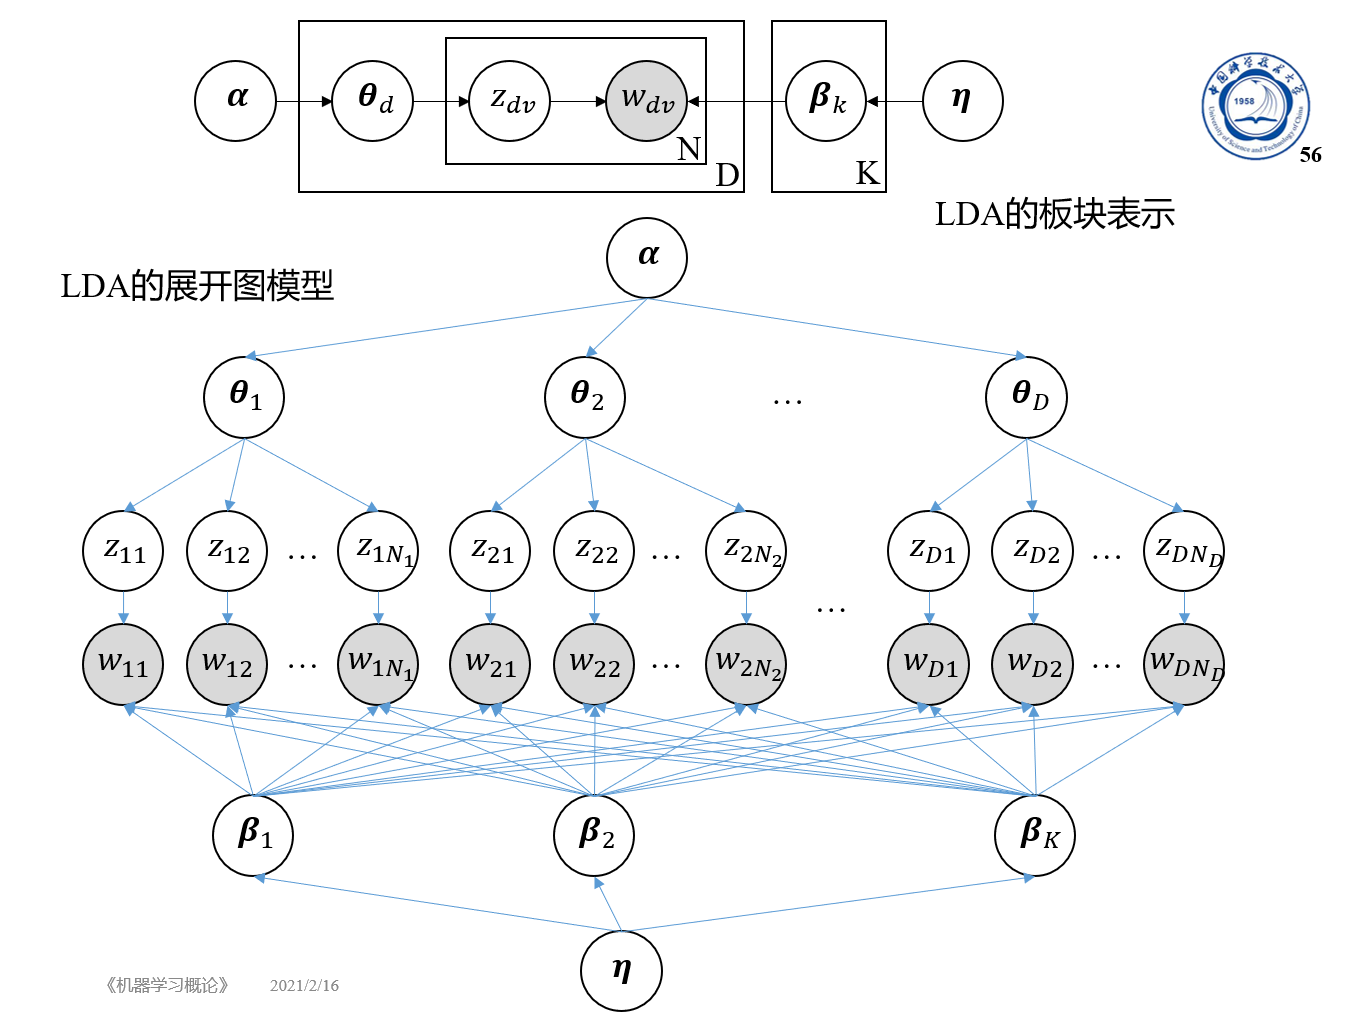
\includegraphics[width=\linewidth/2]{image/lda_diagram.png}
	\caption{LDA 图解(图源自连德富老师的 PPT)}
\end{figure}
\subsubsection{LDA 对应概率分布及求解方式}
有了上述图解, 很容易可以写出来下式
\begin{align}
p(W,z,&\beta,\Theta|\alpha,\eta)=\\
&\prod\limits_{t=1}^Tp(\Theta_t|\bm{\alpha})\prod\limits_{i=1}^Kp(\beta_k|\bm{\eta})\left(\prod\limits_{n=1}^NP(w_{t,n}|z_{t,n},\beta_k)P(z_{t,n}|\Theta_t)\right)
\end{align}
\subsection{Gibbs 采样}
为了对 LDA 模型进行参数估计, 我们可以采用 Gibbs 采样的方法.
\subsubsection{Gibbs 采样算法}
Gibbs 采样可以认为是 Metropolis-Hasting 算法的一个特例. 其算法原理如下:\par
{\centering
\begin{minipage}{\linewidth*5/7}
\begin{algorithm}[H]
\caption{{\sc Gibbs 采样}}
	\begin{algorithmic}[1] %每行显示行号
	\State 初始化 $\{z_i: i=1,\cdots, M\}$
	\For{$\tau = 1,\cdots, T$}
		\State Sample $z_1^{(\tau+1)}\sim p(z_1|z_2^{(\tau)},z_3^{(\tau)},\cdots, z_M^{(\tau)})$
		\State Sample $z_2^{(\tau+1)}\sim p(z_2|z_1^{(\tau+1)},z_3^{(\tau)},\cdots, z_M^{(\tau)})$
		\State $\vdots$
		\State Sample $z_j^{(\tau+1)}\sim
		p(z_j|z_1^{(\tau+1)},\cdots, z_{j-1}^{(\tau+1)},z_{j+1}^{(\tau)},\cdots, z_M^{(\tau)})$
		\State $\vdots$
		\State Sample $z_M^{(\tau+1)}\sim p(z_M|z_1^{(\tau+1)},z_2^{(\tau+1)},\cdots, z_{M-1}^{(\tau+1)})$
	\EndFor
	\end{algorithmic}
\end{algorithm}
\end{minipage}
\par}
\subsubsection{估计 LDA 模型参数}
这一步的过程是
\begin{itemize}
\item 通过对隐变量 $\theta$ 和 $\beta$ 积分, 得到边缘概率 $P(z_d|w_d,\alpha,\eta)$.\\
	由于 $P(z|w,\alpha,\eta)=\frac{P(z|w,\alpha,\eta)}{P(w|\alpha,\eta)}\propto P(z,w,\alpha,\eta)=P(w|z,\alpha,\eta)P(z|\alpha,\eta)=P(w|z,\eta)P(z|\alpha)$, 分别考虑如下积分:
	\begin{equation}
	P(w|z,\eta)=\int p(w|z,\beta)p(\beta|\eta)d\beta=\prod\limits_{k=1}^K\frac{B(\eta+n_k)}{B(\eta)}
	\end{equation}
	\begin{equation}
	p(z|\alpha)=\int p(z|\theta)p(\theta|\alpha)d\theta=\prod\limits_{d=1}^D\frac{B(\alpha+n_d)}{B(\alpha)}
	\end{equation}
	其中, $n_k$ 是一个 $V$ 维向量, $n_{kv}$ 表示数据中第 $k$ 个话题生成第 $v$ 个单词的次数; $n_d$ 是一个 $K$ 维向量, $n_{dk}$ 表示第 $d$ 个文档生成第 $k$ 个主题的次数.
\item 对后验概率进行吉布斯采样, 得到分布 $P(z_d|w_d,\alpha,\eta)$ 的样本集合.
	对于吉布斯采样需要的条件概率, 可以依下式求出:
	\begin{align}P(z_i=k'|z_{-i},\alpha,\eta)&\propto \frac{P(z|w,\alpha, \eta)}{P(z_{-i}|w,\alpha,\eta)}\\
	&=\frac{\eta_{v'}+n_{k'v'}}{\sum_v\eta_v+n_{k'v}}\cdot \frac{\alpha_{k'}+n_{d'k'}}{\sum_k\alpha_k+n_{d'k}}
	\end{align}
\item 估计参数 $\theta_d$ 和 $\beta_k$
	类似地有
	\begin{equation}
	p(\theta_d|z_d,\alpha)\propto\prod\limits_{k=1}^K\theta_{dk}^{\alpha_k-1+n_{dk}}\Rightarrow p(\theta_d|z_d,\alpha)=Dir(\theta_d|n_d+\alpha)\Rightarrow \theta_{dk}=\frac{n_{dk}+\alpha_k}{\sum_k(n_{dk}+\alpha_k)}
	\end{equation}
	同理:
	\begin{equation}
	\beta_{kv}=\frac{n_{kv}+\eta_v}{\sum_v(n_{kv}+\eta_v)}
	\end{equation}
\item 利用这个样本集合对参数 $\alpha$ 和 $\eta$ 进行参数估计.
\end{itemize}
整体的算法可以按如下进行:\par
{\centering
\begin{minipage}{\linewidth*5/7}
\begin{algorithm}[H]
\caption{{\sc LDA 参数估计}}
	\begin{algorithmic}[1]
	\State 为每篇文档的每个词指派一个主题
	\While{未收敛}
		\State 通过 Gibbs 采样对每个 $z_{dv}$ 进行估计.
		\State 根据估计的结果计算 $n_{kv}$ 和 $n_{dk}$, 进而估计参数 $\theta_d$ 和 $\beta_k$
	\EndWhile
	\State \Return $\theta_d$ 和 $\beta_k$
	\end{algorithmic}
\end{algorithm}
\end{minipage}
\par}
\subsubsection{训练终止条件/收敛条件}
显然, 两次抽样结果($z$)的差异能够反应整个训练过程是否趋于稳定. 如果连续两次$\Delta z$ 差异不大, 则说明训练已经趋于收敛:
$$Delta\_Error=\frac{|last\_z - z|}{\sum_{doc}doc\mbox{的词数}} < eps$$


\section{程序概要}
\subsection{数据集介绍}
数据集有
\begin{itemize}
\item 助教给出的 \textbf{text.npy} (一个新闻数据集), 其中包含有 20 个主题, 共有 1000 条文档.
\item 为了验证模型正确性自行构造的 \textbf{cat-computer} 数据集, 其中包含 8 条关于猫这种动物的描述, 6 条关于计算机及其部件的描述. 这些描述主要摘录自 wikipedia. 总共是两个主题, 即\textbf{猫}和\textbf{计算机}.
\end{itemize}

\subsection{预处理}
首先, 考虑到数据集中, 有的文本只包含一些符号, 有的则甚至是空文档. 为了过滤这些, 我调用了 \hlg{langdetect.detect()} 函数来判断文本语言, 从而只保留英文文本.

然后, 又借由 \hlg{sklearn.feature\_extraction.text.CountVectorizer} 来提取字典, 而后通过以下规则进行进一步的过滤:
\begin{itemize}
\item 借助语料库 \hlg{nltk.corpus.brown.tagged\_words()} 尽可能只保留名词
\item 去除标点符号
\item 通过 \hlg{nltk.corpus.stopwords} 过滤停用词
\item 根据一系列正则表达式过滤特殊词
\end{itemize}

\begin{minipage}{\linewidth/2}
\begin{figure}[H]
	\centering
	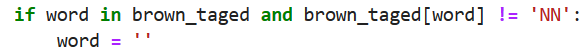
\includegraphics[width=\linewidth]{image/filter_keepnn.png}
	\caption{尽可能保留名词}
\end{figure}
\end{minipage}
\begin{minipage}{\linewidth/2}
\begin{figure}[H]
	\centering
	
\includegraphics[width=\linewidth]{image/filter_punctuations.png}
	\caption{去除的标点符号}
\end{figure}
\end{minipage}\\
\begin{minipage}{\linewidth/2}
\begin{figure}[H]
	\centering
	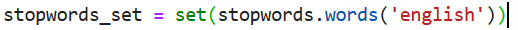
\includegraphics[width=\linewidth]{image/filter_stopwords.png}
	\caption{过滤停用词}
\end{figure}
\end{minipage}
\begin{minipage}{\linewidth/2}
\begin{figure}[H]
	\centering
	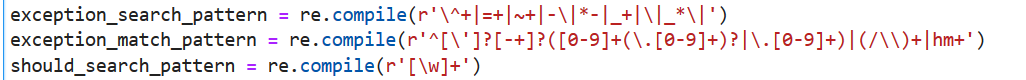
\includegraphics[width=\linewidth]{image/filter_re.png}
	\caption{根据一系列正则表达式过滤}
\end{figure}
\end{minipage}
\jumpLine

经过这些预处理, 整个词库量缩减了很多, 如下表所示:\\
\begin{center}
\begin{tabular}{|c|c|c|c|}
\hline
 & 原文档 & sklearn 预处理 & 进一步过滤 \\
\hline
新闻数据集词汇量 & 28323 & 19285 & 11206 \\
\hline
cat-computer 数据集 & 804 & 745 & 250 \\
\hline
\end{tabular}
\end{center}

最后能够得到一个矩阵表示的文档集, $doc\_vec \in N^{D\times V}$, 每个元素表示对应文档中对应单词出现次数.

\subsection{参数设置}
主要涉及到的参数就是 $\alpha$, $\beta$, $max\_epoch$ 及话题数目. 如下:
\begin{center}
\begin{tabular}{|c|c|c|c|c|}
\hline
 & $\alpha$ & $\beta$ & $max\_epoch$ & 话题数 \\
\hline
新闻数据集 & 均0.01 & 均0.01 & 1000 & 20 \\
\hline
cat-computer 数据集 & 均0.01 & 均0.01 & 100 & 2 \\
\hline
\end{tabular}
\end{center}
\section{实验结果}
由于还有自己做的一个小数据集 Cat-Computer 数据集, 这里先以定性的角度分析一下该数据集的结果, 然后在下一部分中, 再定性+定量地分析一下新闻数据集的结果.
\subsection{Cat-Computer 数据集}
\begin{center}
\begin{figure}[H]
	\centering
	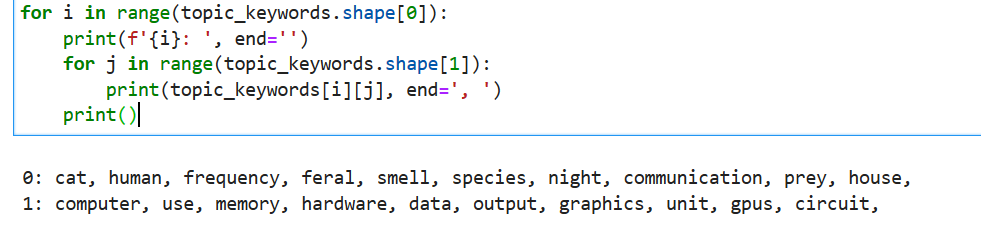
\includegraphics[width=\linewidth]{image/ccresult.png}
	\caption{Cat-Computer 数据集实验结果}
\end{figure}
\end{center}
可以看到这里面两个话题的关键词都非常的准确, 具体而言:
\begin{itemize}
\item Cat 类话题关键词: 猫, 人, 野生的, 嗅觉, 物种, 夜晚, 交流, 猎物 等词汇都能很好地体现这个话题
\item Computer 类话题关键词: 计算机, 内存, 硬件, 数据, 输出, 图形的, 单元, GPU, 电路等词汇都完美地体现了计算机这一主题.
\end{itemize}
在小数据集上, 可以发现 LDA 模型表现非常的优秀, 因此我们基本可以断定, 这个程序是能够正常运行, 并给出对应话题及其相关的关键词的. 于是我们就可以进一步探究本实验给出的官方数据集——新闻数据集.
\subsection{新闻数据集}
\subsubsection{训练过程曲线}
整个训练过程中, 为了观察模型是否收敛, 我们优先考虑了连续两次模型预测结果的差异, 同时也参考 $\theta$ 和 $\beta$ 的变化. 经过统计及可视化, 可以得到如下图表:
\\\noindent
\begin{center}
\begin{figure}[H]
	\centering
	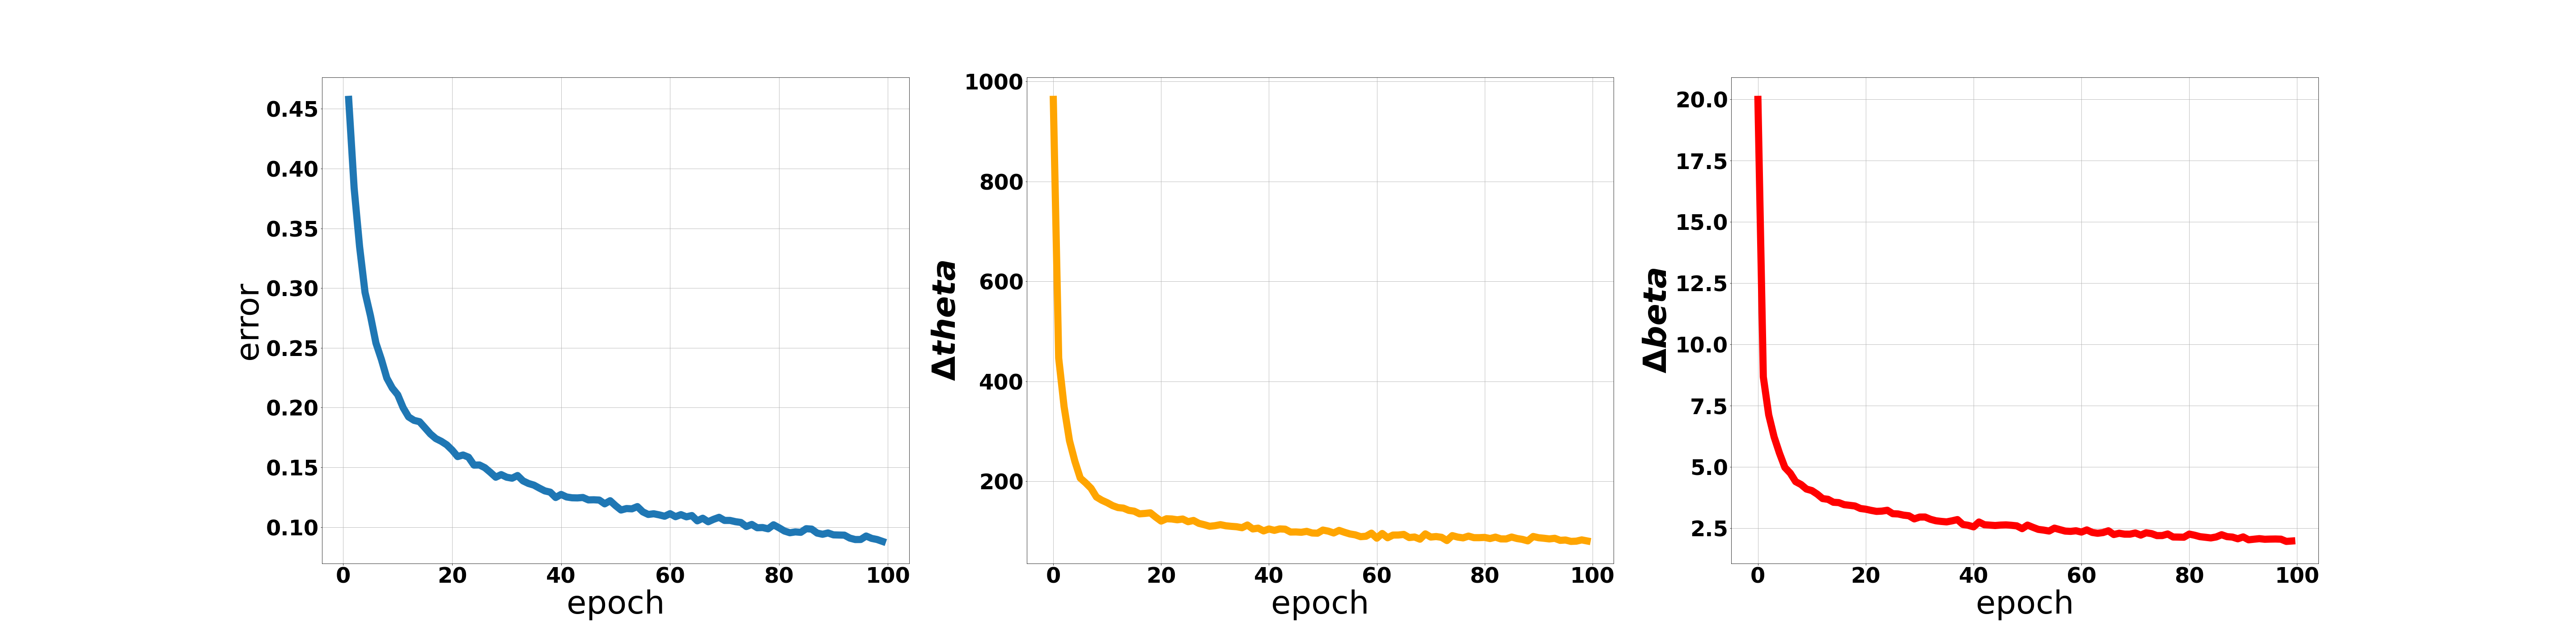
\includegraphics[width=\linewidth]{image/newstraining.png}
	\caption{新闻数据集训练过程, 左图为连续两次模型预测结果的差异, 中图为 $\theta$ 的变化, 右图为 $\beta$ 的变化}
\end{figure}
\end{center}

很显然, 这三个值都呈指数级下降的趋势, 说明我们的训练过程是非常有效的. 值得注意的是, 最终 error 低达 0.10, 这意味着两次之间的词汇到话题的预测只有 0.10 的差异. 而反映了文档中话题的分布情况的 $\theta$ 及反映话题中关键词分布情况的 $\beta$ 也都趋于稳定. 其中, 值得说明的是:
\begin{itemize}
\item $\theta$ 差异趋于 80 左右, 这说明 1000 篇文档的话题分布中, 只有 8\% 的话题分布不太稳定
\item $\beta$ 差异趋于 2.0 左右, 这说明 20 个话题中只有 2\% 的关键词分布不太稳定
\end{itemize}
\subsubsection{话题的关键词结果说明}
下图是 news 数据集的训练结果, 每一行是 10 个关键词, 表示了该话题的 top10 关键词.
\begin{center}
\begin{figure}[H]
	\centering
	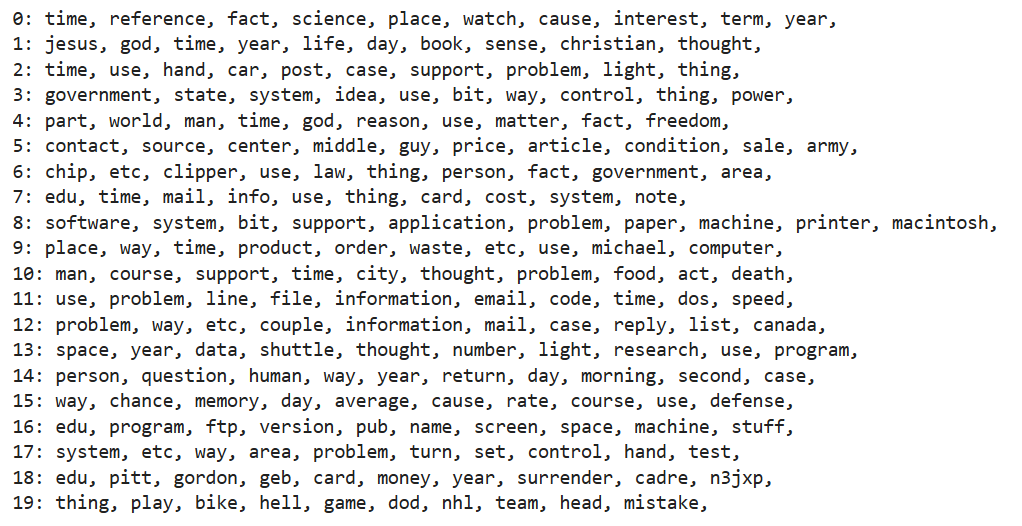
\includegraphics[width=\linewidth*7/9]{image/newsresult.png}
	\caption{新闻数据集结果}
\end{figure}
\end{center}

可以看到, 里面虽然有部分话题的含义比较模糊不清, 但有一些比较突出的值得说明一下:
\begin{itemize}
\item 0号话题中的: 时间, 引用, 事实, 科学, 原因等词汇能够反映\textbf{科学}这一话题
\item 1号话题中的: 耶稣, 上帝, 生命, 基督, 书籍等词汇能够反映\textbf{宗教信仰}这一话题
\item 3号话题中的: 政府, 国家, 制度, 理念, 控制, 权力等词汇能够反映\textbf{政治}这一话题
\item 7号话题中的: edu, 时间, 邮件, 信息等词汇能够反映\textbf{邮件/电子邮件}这一文本背景. 识别出这样的东西是很合理的, 因为数据集中出现了大量的邮件文本.
\item 8号话题中的: 软件, 系统, 比特, 支持, 应用, 问题, 论文, 机器, 打印机, Macintosh(苹果公司早年电脑型号) 就完美地适配了\textbf{电脑/计算机}这一主题
\item 9号话题中的: 产品, 订单, 位置等词汇能够一定程度地体现\textbf{商业}话题
\item 13号话题中的: 太空, 年, 数据, 航天飞机, 思考, 数字, 光, 研究, 使用, 计划等词汇则可以反映\textbf{航天}这一话题
\item 19号话题中的: 事件, 运动, 自行车, 比赛, 国家冰球联盟, 团队, 领导, 错误等词汇则可以反映\textbf{体育赛事}
\end{itemize}
\subsubsection{文档分类结果说明}
通过以下代码我们可以找出, 每个话题中最具代表性的文本. 由于 theta 每行表示对应文档的话题分布, 因此找 theta 每列最值的索引, 可以给出每个话题最具代表性的文本. 其中输出结果第一行是每个话题对应最具代表性的文本, 比如 687 是话题 1 最具代表性的文本, 而第二三行是其对应概率, 这里为 0.916.
\begin{center}
\begin{figure}[H]
	\centering
	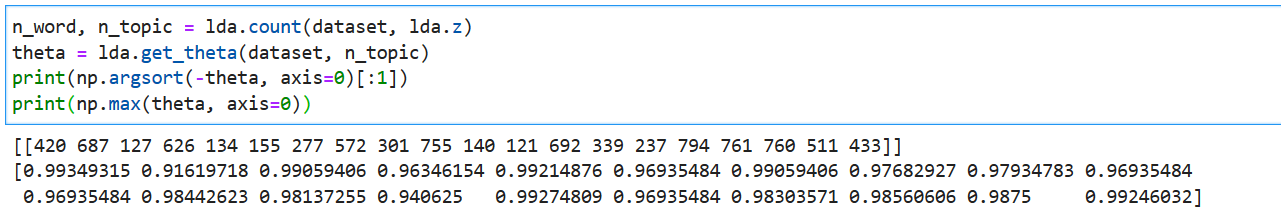
\includegraphics[width=\linewidth]{image/doctopic.png}
	\caption{获取每个话题中最具代表性的文本}
\end{figure}
\end{center}
下面举两个例子说明:
\begin{enumerate}[1. ]
\item 例子1: 上一节中, 我们提到 1 号话题与宗教信仰关联, 输出其对应最具代表性的文档, 会发现它是关于"启示录"中12:7-9的内容, 见图\ref{topic1doc}.
\item 例子2: 话题19对应的是体育赛事, 可以发现对应最具代表性的文档如下, 是一个体育赛事的记分榜之类的文本, 见图\ref{topic19doc}.
\end{enumerate}
\begin{minipage}{\linewidth/2}
\begin{figure}[H]
	\centering
	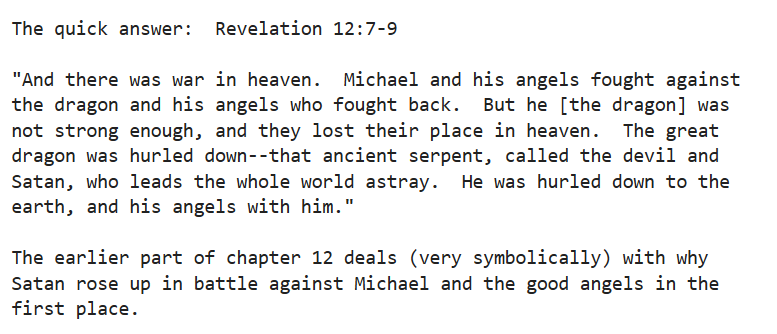
\includegraphics[width=\linewidth]{image/topic1doc.png}
	\caption{最可能是1号话题(宗教信仰话题)的文本}
	\label{topic1doc}
\end{figure}
\end{minipage}
\begin{minipage}{\linewidth/2}
\begin{figure}[H]
	\centering
	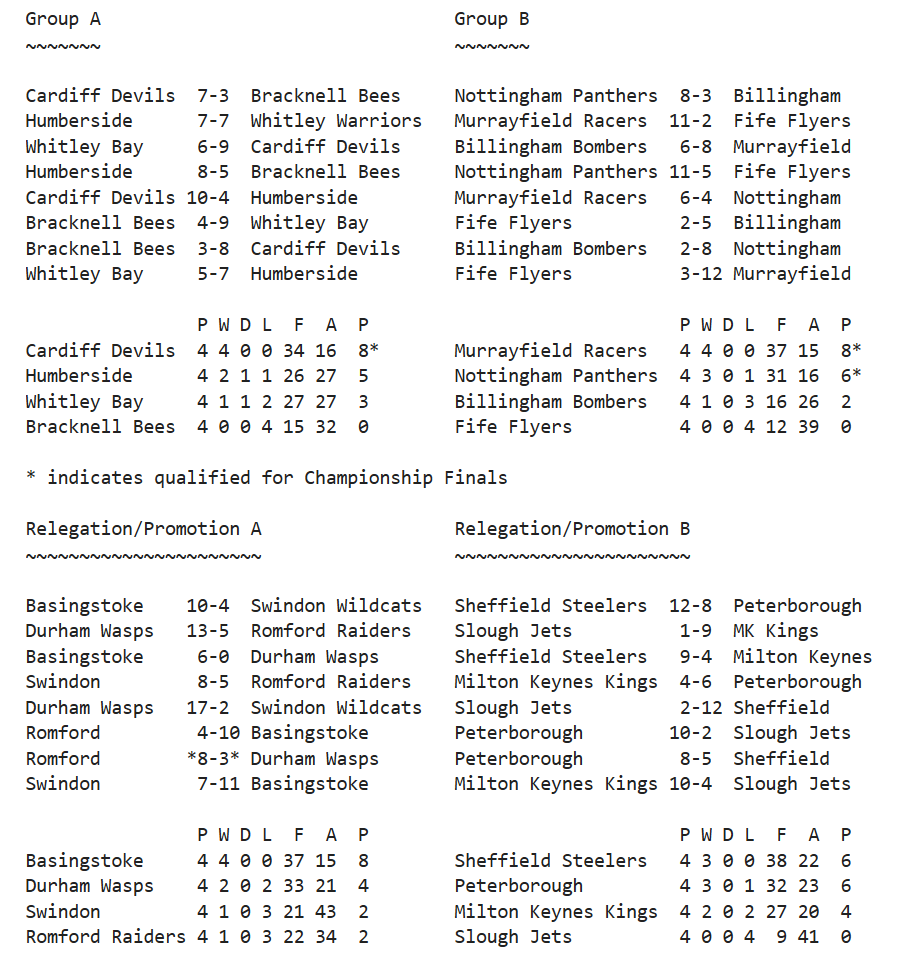
\includegraphics[width=\linewidth]{image/topic19doc.png}
	\caption{最可能是19号话题(体育赛事话题)的文本}
	\label{topic19doc}
\end{figure}
\end{minipage}

\section{实验总结}
本次 LDA 实验通过一个新闻数据集, 让我深刻理解了 LDA 算法原理与流程. 令我震惊的是, 这个话题模型甚至能够识别出记分榜这样的数据, 这说明本次实验完成的模型是非常有效的.



	
\end{document}